\section{简介}
一个希望在远端执行计算的用户面临一个复杂的tradeoff:能够在多大程度上相信远端的系统?为了安全愿意付出多大的性能开销?远端系统可以抵御多强的攻击者?一个理想系统应该能够在保证可信隐私计算的同时不引入性能开销、TCB为零,当然这样的理想系统是不存在的。

一个极端情况就是引入开销很大的加密技术,通过引入高昂的代价实现\textbf{无信任计算}(\textit{trust-free computation})。依赖另一种极端情况的云计算场景:假设能够不用检查地信任远端系统,那么弱安全保证可以以最小的开销实现。这篇文章的目的是说明对远端系统适度信任的情况下可以实现一些重要的安全特性。 一系列安全处理器探索了可信硬件的空间,使得能够应对各种威胁模型的廉价远端计算成为可能。

关于安全的严谨的探讨需要精确地描述威胁模型:可新硬件必须安全意味着它必须有针对明确指定的威胁模型的适应能力。比如针对有能力对系统硬件进行物理篡改的攻击者,很少有系统能够提供有意义的安全保证。虽然符合“安全处理器”描述的范围确实很大,但是这篇工作集中在能够实现\textbf{安全远端计算}(\textit{secure remote computation})的系统。具体来说,这篇工作旨在阐明于\textit{enclave}相关的编程模型、历史背景、设计决策以及威胁模型,其中\textit{enclave}是最新而且是目前最安全的安全远端计算系统。我们调研了Intel的Software Guard Extensions(SGX)以及MIT的Sanctum系统来对有\textit{enclave}能力的系统进行举例说明。

\subsection{安全远端计算}

安全远端计算(图 \ref{SecureRemoteComputation})是指在不可信三方拥有或者维护的远端计算机上运行软件,同时要在一定程度上保证\textbf{完整性}(\textit{integrity })和\textbf{私密性}(\textit{confidentiality})的问题。在普通配置下,安全远端计算是个尚未解决的问题。完全的\textbf{同态加密}(\textit{Homomorphic Encryption})只是在有限几种计算上解决了这个问题,同时还引入了非常巨大的性能开销。
% fiture
\begin{figure}
\centering
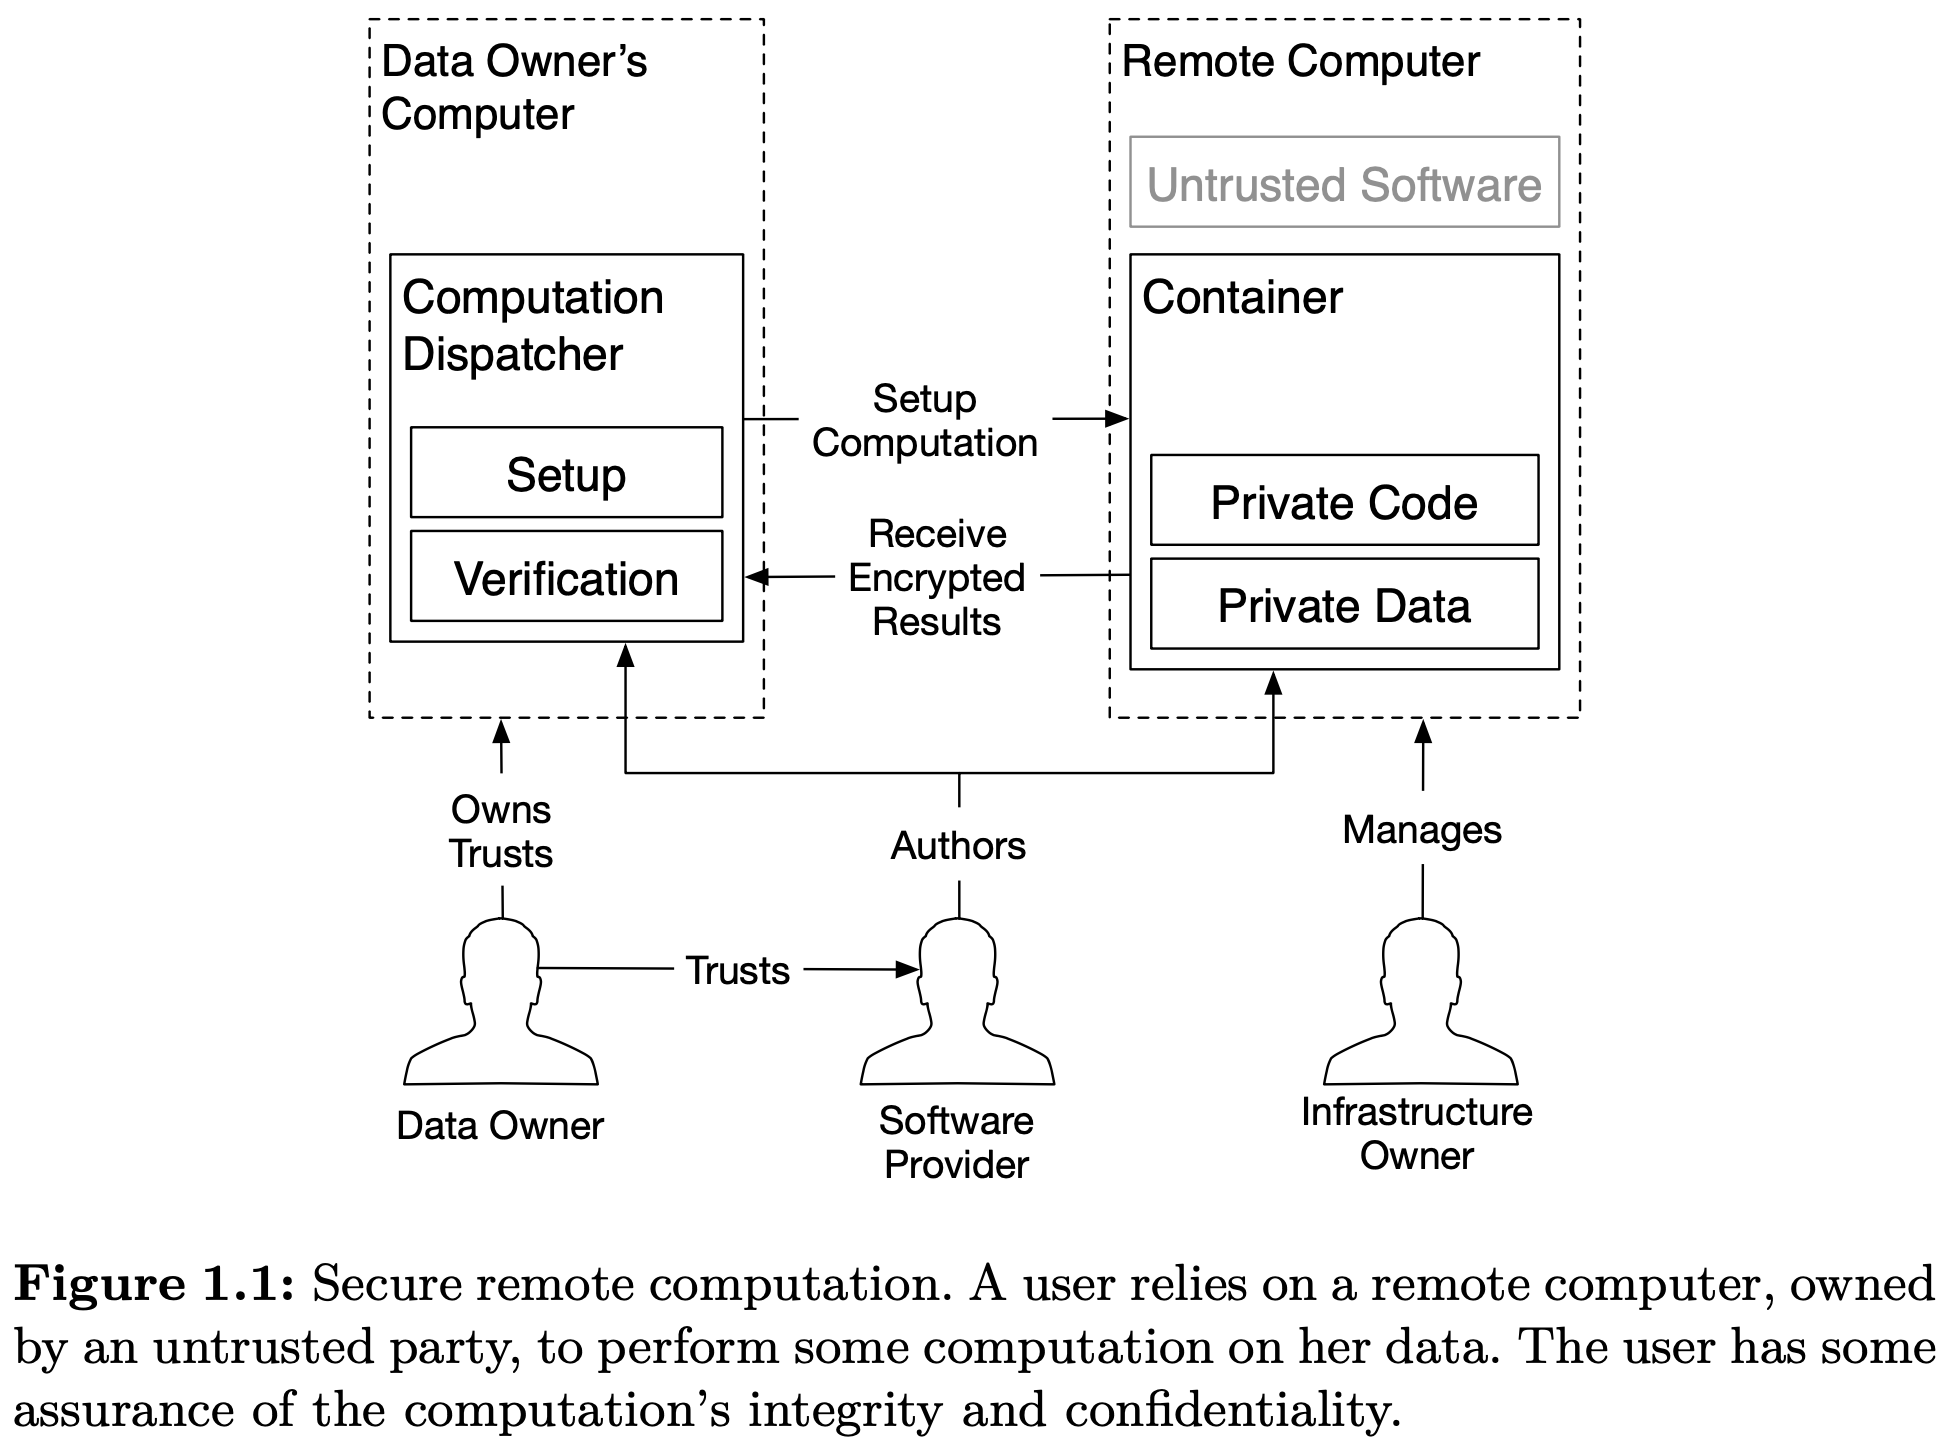
\includegraphics[width=0.8\textwidth]{SecureRemoteComputation.png}
\caption{安全远端计算}
\label{SecureRemoteComputation}
\end{figure}

在很长一系列的可信计算(图\ref{TrustedComputing})设计中,Intel的SGX是最新一次的迭代,它旨在利用远端机器上的可信硬件解决安全远端计算的问题。这种可信硬件建立了一个容器,用户将希望进行的计算和数据上传到这个容器中。在计算执行的过程中,可信硬件保护数据的私密性和完整性。

% fiture
\begin{figure}
\centering
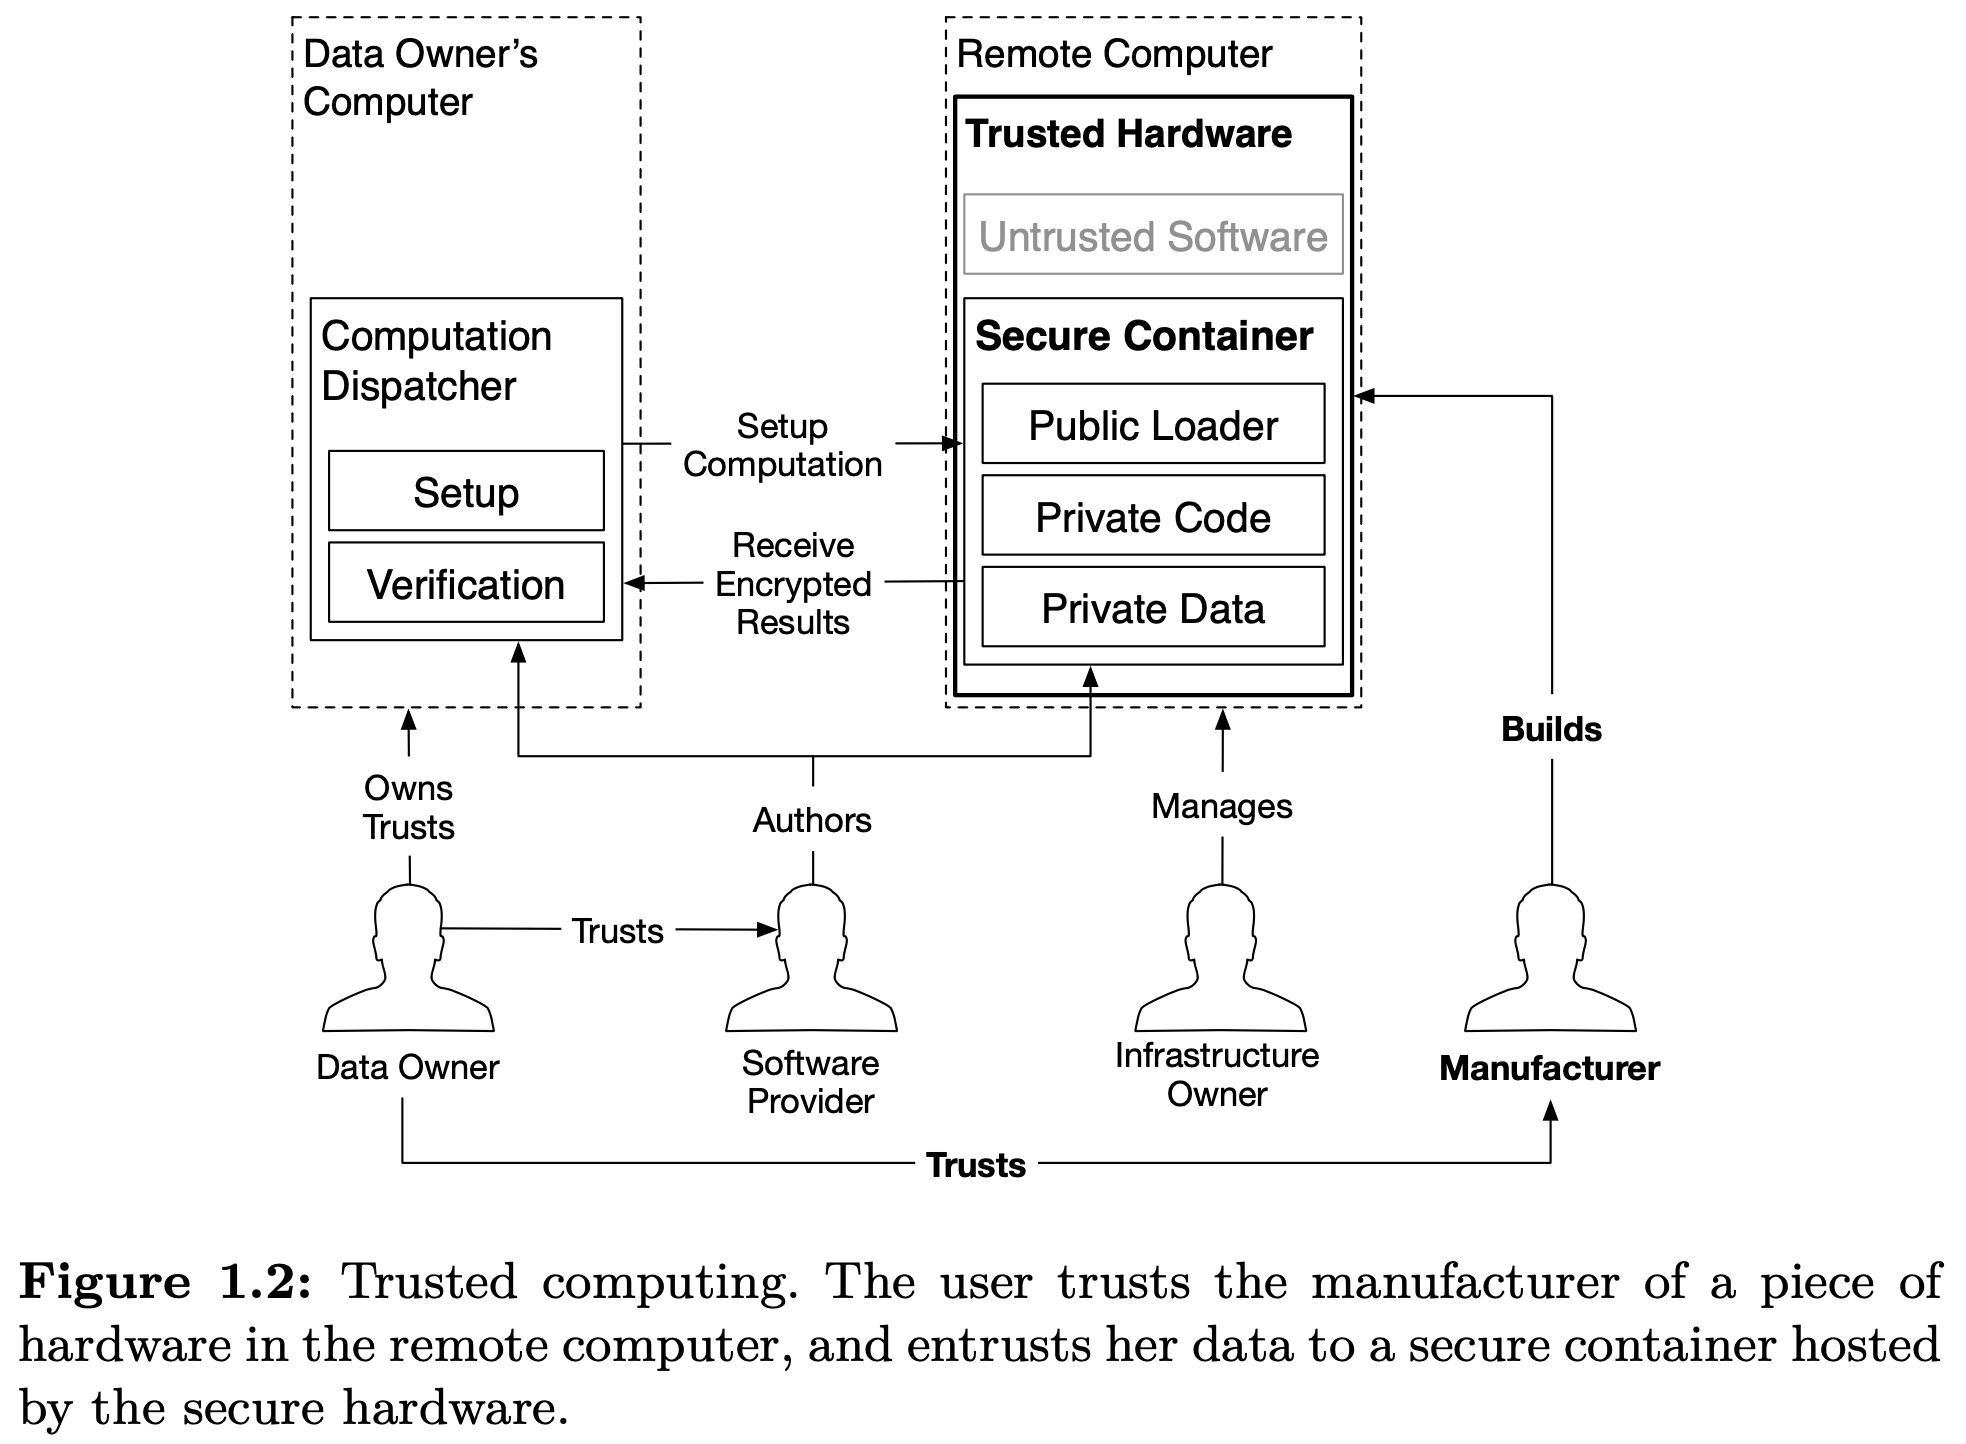
\includegraphics[width=0.8\textwidth]{TrustedComputing.png}
\caption{可信计算}
\label{TrustedComputing}
\end{figure}

SGX、Sanctum这类工作和它们之前的工作(比如TPM和TXT)一样都依赖于\textbf{软件验证}(\textit{software attestation})。软件验证(图\ref{SoftwareAttestation})向用户证明它正在与可信硬件支持的安全容器中运行的特定软件进行通信。这个证明是一个加密签名,它能证明安全容器中内容的哈希的正确性。\textbf{它遵循的原则是:远端计算机的拥有者可以向安全容器中加载任意的软件,同时安全容器中内容的哈希和用户期望的不相符时,用户也可以拒绝将隐私数据上传。}

% fiture
\begin{figure}
\centering
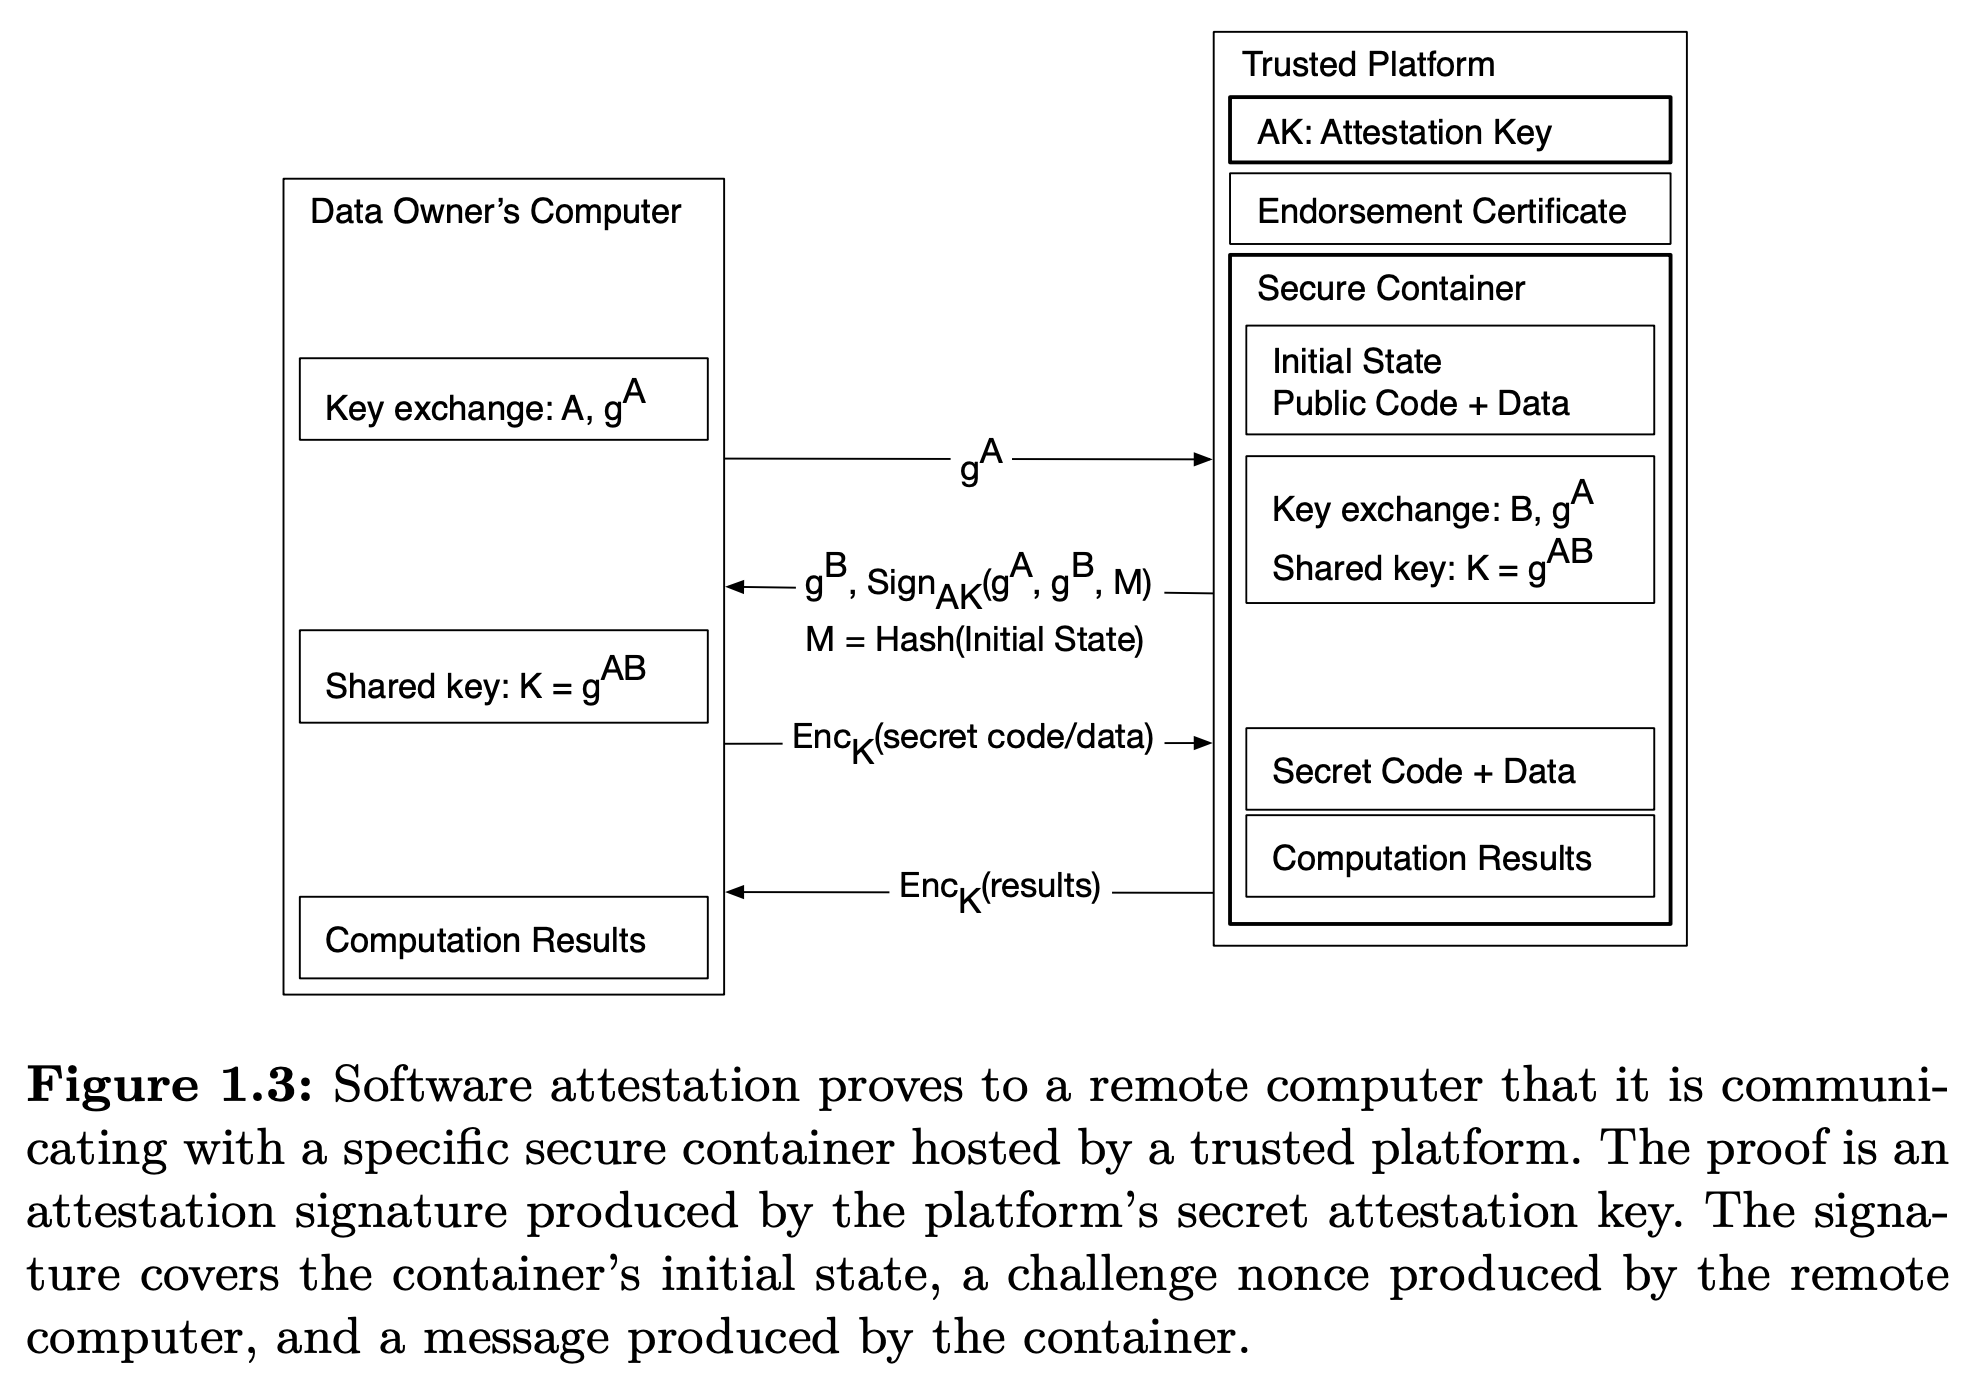
\includegraphics[width=0.8\textwidth]{SoftwareAttestation.png}
\caption{软件验证}
\label{SoftwareAttestation}
\end{figure}

用户根据由可信硬件制造商(这里是Intel)创建的证书来验证用于产生签名的\textbf{证明密钥}(\textit{attestation key})。证书表明只有可信硬件知道证明密钥,并且仅用于证明目的。

SGX之所以能从它的前任工作中脱颖而出,主要原因在于验证覆盖的代码数量,这些代码是在硬件保护的系统的TCB(\textit{Trusted Computing Base})中的。在原始TPM的设计中产生的验证覆盖了运行在计算机上的所有软件;TXT中验证覆盖了一个VMX虚拟机中的代码。而在SGX中,一个\textit{enclave}(安全容器)只包含计算中需要的隐私数据以及操作它的代码。

比如,一个处理医疗图像的云服务的实现中,可能需要拥有用户上传的加密过的医疗图像。用户会把用于加密的密钥发送给运行在\textit{enclave}中的软件。软件中可能包含解密图像的代码、处理图像的算法以及加密结果的代码。而接受上传的加密图像并存储图像的代码会被放在\textit{enclave}之外。图\ref{ExampleSoftwareInSGX}描述了这个例子

\begin{figure}
\centering
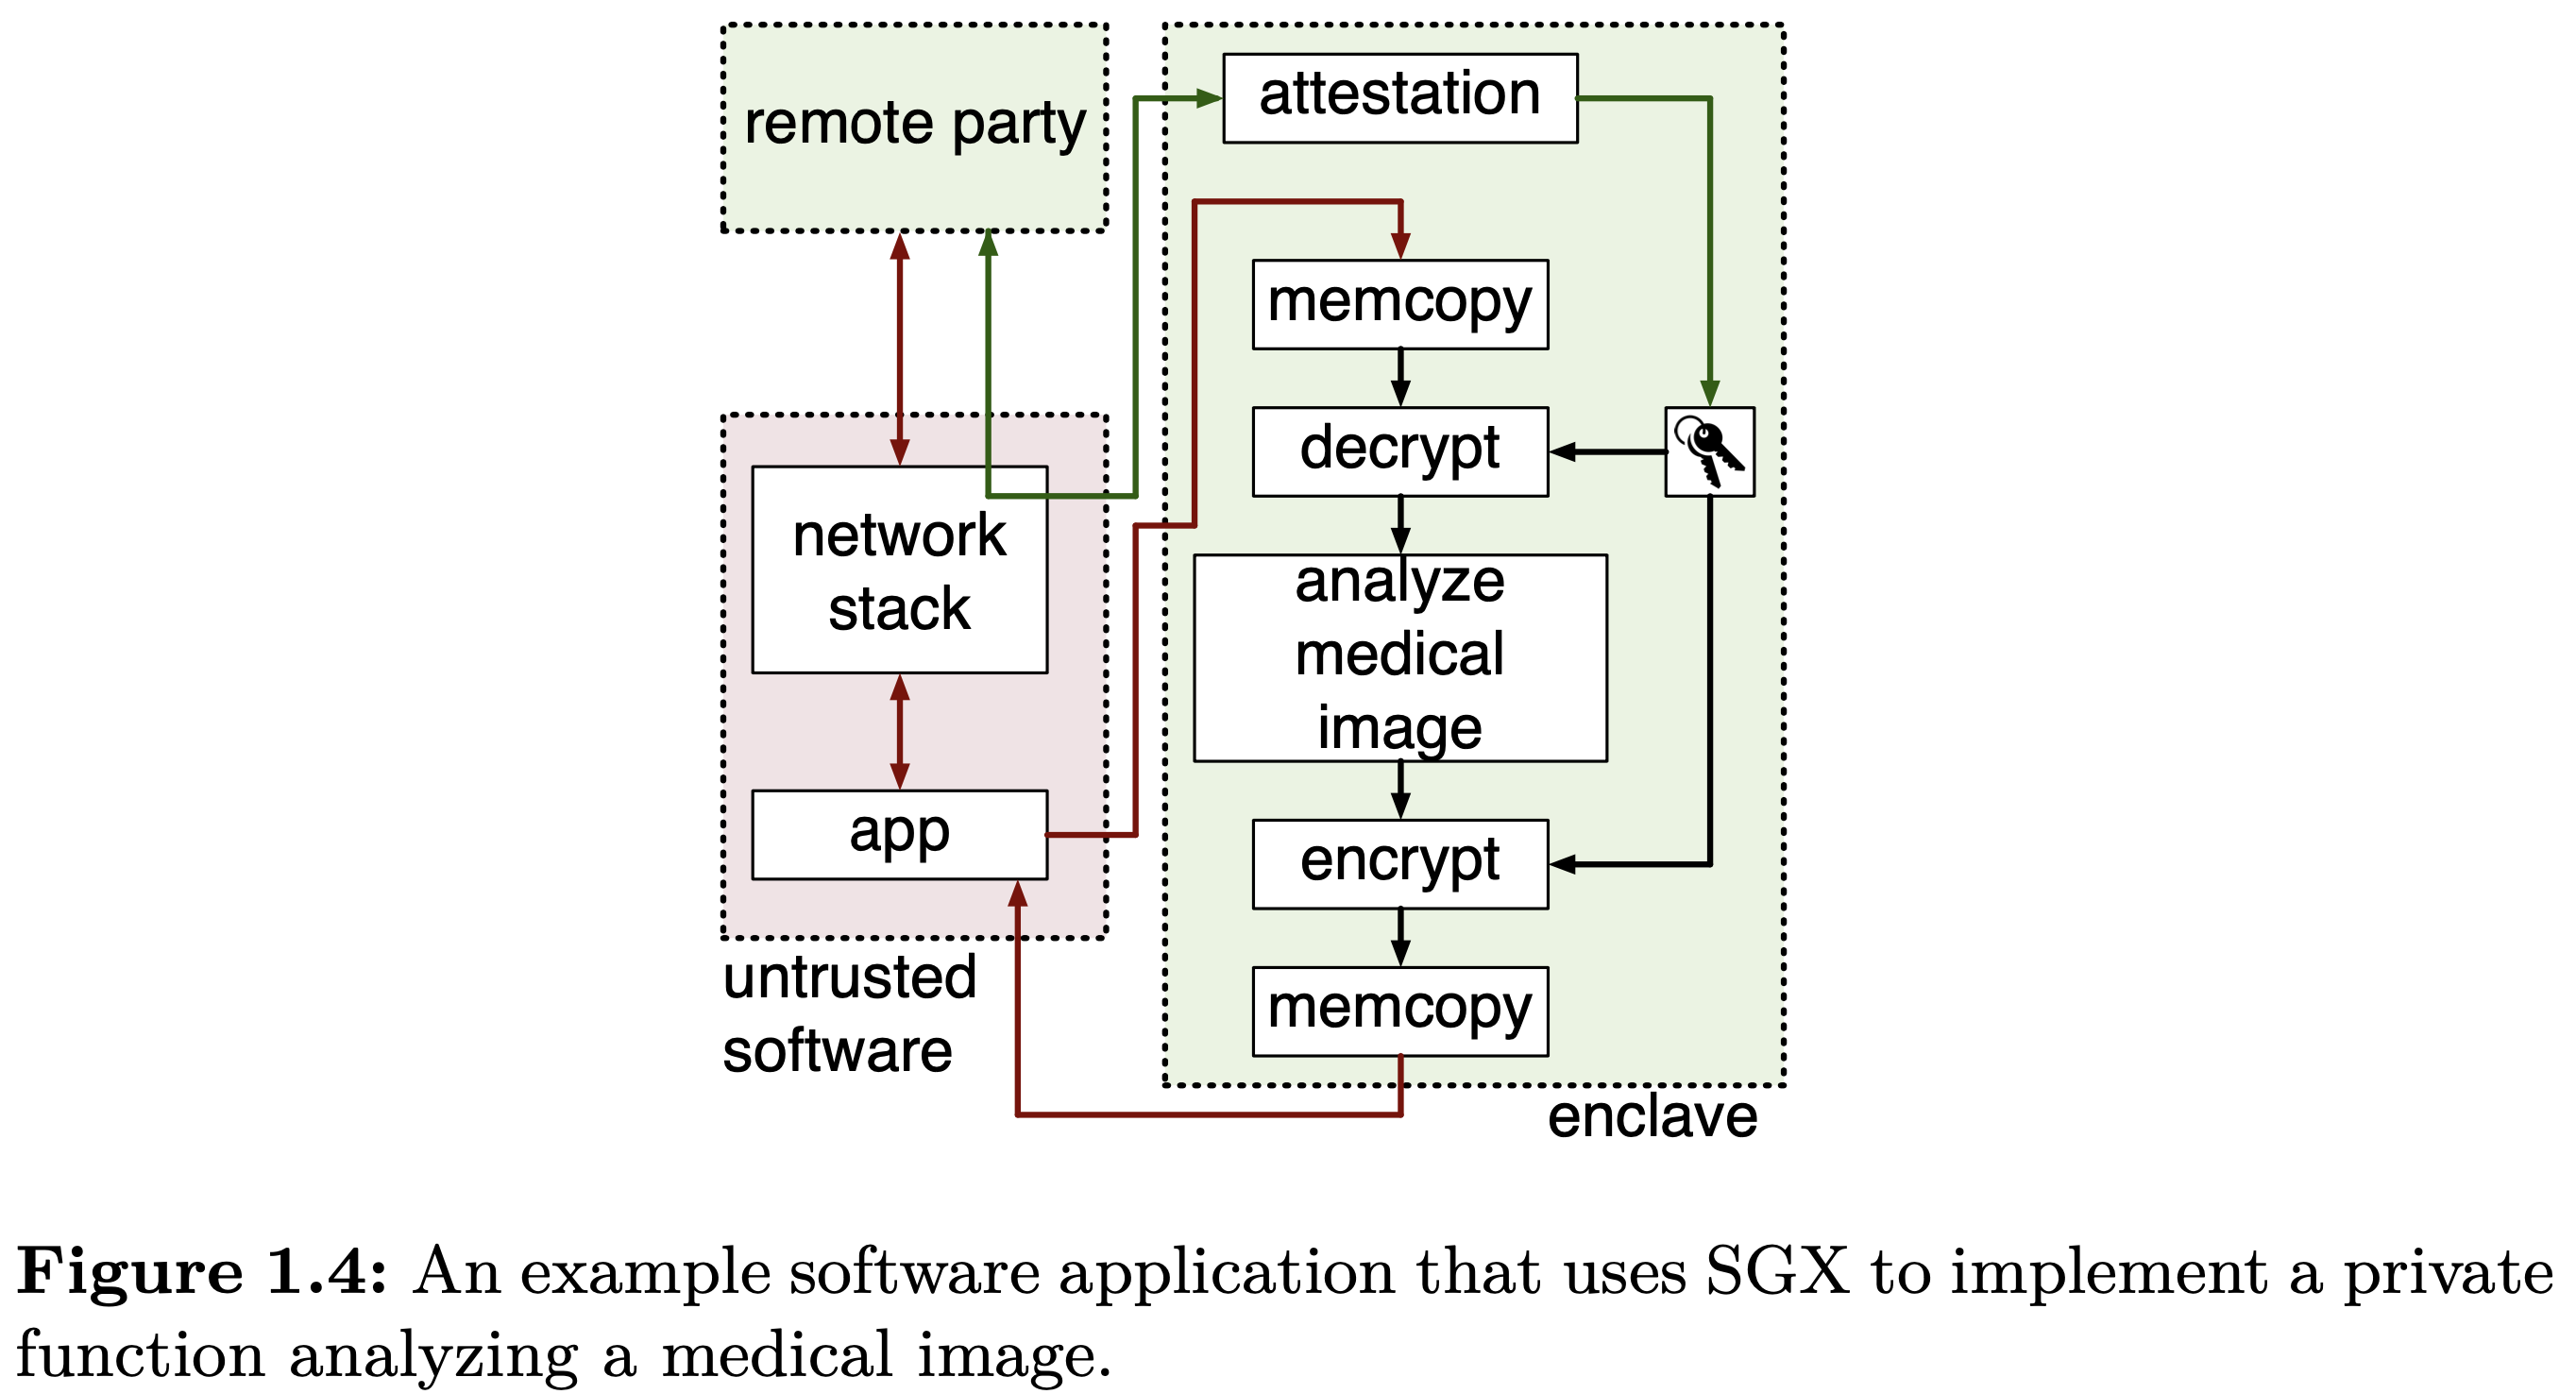
\includegraphics[width=0.8\textwidth]{ExampleSoftwareInSGX.png}
\caption{运行在SGX中的一个软件}
\label{ExampleSoftwareInSGX}
\end{figure}

支持\textit{enclave}的处理器通过将\textit{enclave}的数据和代码与其他软件隔离开来保证\textit{enclave}中计算的完整性和私密性,这里的其他软件不光包括用户软件也包括OS/Hypervisor以及连接到总线上的硬件设备。同时SGX模型保持了Intel传统架构中软件层次的兼容,在Intel传统架构中OS kernel和Hepervisor负责管理计算机资源。

本文将会讨论SGX的初始版本,我们称之为SGX 1。尽管SGX 2位\textit{enclave}开发者带来了非常有用的改进,但是从设计和实施的角度来看,SGX 2只是一个小的渐进式的改进。理解SGX 1背后的原理和它的安全特性之后,读者们应该具备足够的知识来应对Intel的参考文档,并且学习SGX 2和最近工作带来的改变。

\subsection{对SGX简单概述}
尽管这份手稿是想教会读者执行远端计算的安全处理器的挑战、历史以及最先进技术,但是相关讨论是以Intel的SGX为例子展开的,因为它是目前可得的、提供文档的、旨在为远端执行软件提供有用安全保证的现代系统。这一部分是关于SGX的一个简单概述,引导读者阅读手稿的其他部分,以深入了解SGX的各个方面。

SGX留住一块内存区域,成为\textbf{PRM}(\textit{Processor Reserved Memory})。CPU保护PRM,使其不能被非\textit{enclave}的内存访问,包括OS kernel、Hypervisor以及外围管理引擎。

PRM中包含\textbf{EPC}(\textit{Enclave Page Cache}),EPC由4KB的页组成,用于存储\textit{enclave}的代码和数据。不被信任的系统软件负责给\textit{enclave}分配EPC页。CPU在\textbf{EPCM}(\textit{Enclave Page Cache Metadata})中追踪每个EPC页的状态,以保证每个EPC页不会被重复分配并且只会属于唯一的\textit{enclave}。

\textit{enclave}中的初始代码和数据是由不可信的系统软件加载的。在加载过程中系统软件请求CPU将PRM外的不受保护的内存中的指定数据复制到EPC页中,并将这些EPC页分配给正在设置中的\textit{enclave}。这意味着系统软件是知道\textit{enclave}的初始状态的。

\textit{enclave}的页被加载到EPC中之后,系统软件请求CPU将\textit{enclave}标记为已初始化。在这之后应用程序软件才可能在\textit{enclave}内执行代码。在\textit{enclave}完成初始化以后,上面简单介绍的加载机制已经不能被系统软件使用了。

在\textit{enclave}的加载过程中,它的内容和相关配置会被CPU加密哈希(\textit{cryptographically hash})。当\textit{enclave}初始化完成时,这个哈希值被最终确定下来了,成为\textit{enclave}的\textbf{度量哈希}(\textit{measurement hash})。

位于远端的参与者可以与\textit{enclave}通信执行软件验证以确认它是在和拥有特定度量哈希并且运行在安全环境中的\textit{enclave}在通信。

执行流(\textit{execution flow})只能通过特殊的CPU指令进入\textit{enclave},类似于在经典系统中执行的用户态和内核态之间的模式转换机制。\textbf{\textit{enclave}必须运行在用户态(ring 3)保护模式(\textit{protected mode})下,并且使用由OS kernel/Hypervisor设置的虚拟地址转换。}

为了避免泄露隐私信息,在CPU中执行的\textit{enclave}代码不会直接服务任何中断、错误以及VM退出,而是由CPU执行AEX(\textit{Asynchronous Enclave Exit})实现从\textit{enclave}代码到ring 3代码的切换,然后在给定清除故障信息的情况下处理中断,错误或VM退出。CPU执行AEX就是把CPU状态保存到提前定义好的\textit{enclave}中的一块区域中,然后将控制权转移到提前定义好的\textit{enclave}外的地址空间,并且将向CPU寄存器填充编造的数据。

为\textit{enclave}分配EPC页的任务是由OS kernel或者Hypervisor完成的。OS通过特殊的内核态CPU指令将其起分配决定传送给SGX平台。OS还可以驱逐EPC页,并将其放在不可信的的DRAM中,后面再将起加载进来,这个过程也是通过特殊的内核态CPU指令完成的。SGX通过加密机制实现被驱逐EPC页(驱逐后放在不可信的DRAM中)的私密性、完整性和时新性。

\subsection{概述}

推断Intel SGX的安全特性需要大量的背景知识,这些背景知识很分散。所以本工作的很大部分是收集这些必备知识。下面的几章中会分别介绍相关知识。
